\documentclass[11pt, a4paper]{article}
\usepackage[letterpaper, portrait, margin=0.5in]{geometry}
\usepackage[english]{babel}  % force American English hyphenation patterns
\usepackage{amsmath,mathtools}

\usepackage{graphicx}
\usepackage{wrapfig}


\begin{document}
\title{Chapter 26 Direct-Current Circuits}
\author{Apostolos Delis}
\date{\today}
\maketitle

\tableofcontents
\section[26.1 Resistors In Series and Parallel]{Resistors In Series and Parallel}
\begin{itemize}
    \item \textbf{Direct Current Circuits (DC)}: direction of the current does not
        change with time
    \item \textbf{Alternating Current Circuits (AC)}: the current oscillates back and fort
    \item For any combination of resistors we can always find a single resistor that
        could replace the combination and result in the same total current and potential
        difference
    \item The resistance of this single resistor is called the \textbf{equivalent
            resistance} of the combination.
        \begin{equation}
            V_{ab} = IR_{eq} \; \; \; \text{or} \; \; \; R_{eq} = \frac{V_{ab}}{I}
        \end{equation}
        where $V_{ab}$ is the potential difference between terminals $a$ and $b$ in the
        network and $I$ is the current at point $a$ or $b$
\end{itemize}

\subsection{Resistors in Series}
\begin{itemize}
    \item When resistors are in series, the current $I$ is the same in all of them.
        Applying $V = IR$ to each resistor, with $R_1$, $R_{2}$ and $R_{3}$, we have
        \begin{align}
            V_{ax} = IR_{1} && V_{xy} = IR_{2} && V_{yb} = IR_{3}
        \end{align}
    \item The potential differences across each resistor don't need to be the same, . The
        potential difference $V_{ab}$ across the entire combination is the sum of these
        individual potential differences
        \begin{equation}
            V_{ab} = V_{ax} + V_{xy} + V_{yb} = I(R_{1} + R_{2} + R_{3})
        \end{equation}
        and so:
        \begin{equation}
            \frac{V_{ab}}{I} = R_{1} + R_{2} + R_{3}
        \end{equation}
    \item The Ration $V_{ab} / I$ is the equivalent resistance $R_{eq}$. So
        \begin{equation}
            R_{eq} = R_{1} + R_{2} + R_{3}
        \end{equation}
        This of course can be generalized for any $n$ number of resistors,
        \begin{equation}
            R_{eq} = R_{1} + R_{2} + R_{3} + \cdots + R_{n}
        \end{equation}
\end{itemize}

\subsection{Resistors in Parallel}
\begin{itemize}
    \item If the resistors are in parallel, the current through each resistor does not
        have to be the same. Suppose there are three resistors, with currents $I_{1}$,
        $I_{2}$, and $I_{3}$, then:
        \begin{align}
            I_{1} = \frac{V_{ab}}{R_{1}} && I_{2} = \frac{V_{ab}}{R_{2}} &&
            I_{3} = \frac{V_{ab}}{R_{3}}
        \end{align}
    \item Because charge neither accumulates at nor drains out of point a, the total
        current I must equal the sum of the three currents in the resistors:
        \begin{equation}
            I = I_{1} + I_{2} + I_{3} =
            V_{ab}\bigg(\frac{1}{R_1} + \frac{1}{R_{2}} + \frac{1}{R_3}\bigg)
            \; \; \; \text{or} \; \; \;
            \frac{I}{V_{ab}} = \frac{1}{R_1} + \frac{1}{R_{2}} + \frac{1}{R_3}
        \end{equation}
    \item Then for any $n$ number of resistors in parallel, we have that the equivalent
        resistance $R_{eq}$ is:
        \begin{equation}
            R_{eq} = \frac{1}{R_1} + \frac{1}{R_2} + \frac{1}{R_{3}}
        \end{equation}
\end{itemize}

\section[26.2, Kirchhoff's Rules]{Kirchhoff's Rules}
\begin{itemize}
    \item Many practical resistor networks cannot be reduced to simple series-parallel
        combinations
    \item A \textbf{Junction} in a circuit is a point where three or more conductors meet
    \item A \textbf{Loop} is any closed conducting path
    \item For Junctions, Kirchhoff's rule states that the sum of the current must equal 0
        \begin{equation}
            \sum I = 0
        \end{equation}
        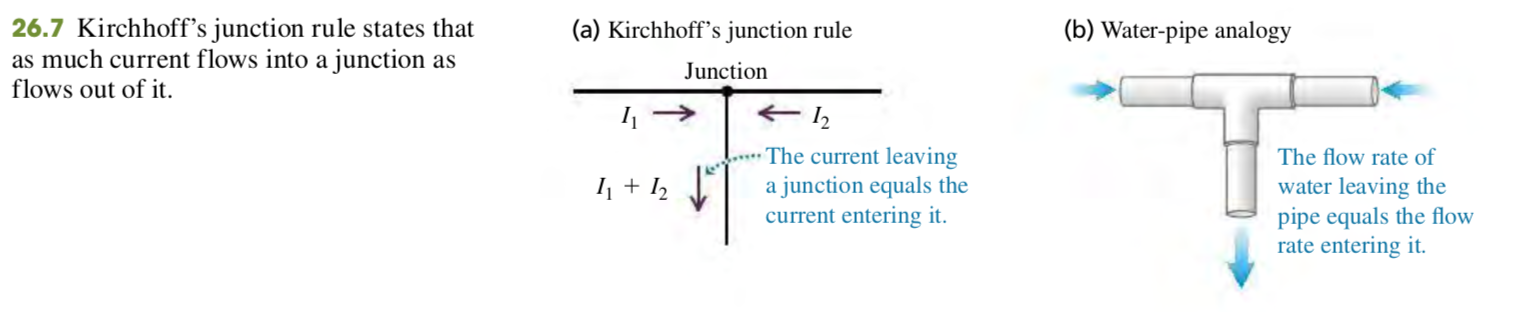
\includegraphics[scale=0.65]{images/junction_rule.png}
    \item For loops, Kirchhoff's rule states that the sum of the potential differences
        around any loop must equal 0
        \begin{equation}
            \sum V = 0
        \end{equation}
    \item The loop rule is a statement that the electrostatic force is conservative.
\end{itemize}

\section[26.3, Electrical Measuring Instruments]{Electrical Measuring Instruments}
\begin{itemize}
    \item \textbf{Ammeters}: current-measuring instruments that measure how much current
        is passing through them. An ideal Ammeter has zero resistance, but real ammeters
        always have as little resistance as possible.
    \item Ammeters can be added to a circuit to measure currents larger than its full
        scale by connecting a resistor in parallel, so that some of the current bypasses
        the meter coil. The parallel resistor is called the \textbf{shunt resistor}
        $R_{sh}$
    \item \textbf{Voltmeters}: are voltage-measuring instruments that measures the
        potential difference between two points. Real voltmeters always have finite
        resistance, but a voltmeter should have large enough resistance that connecting
        it in a circuit does not change the other currents appreciably.
    \item A voltmeter and an ammeter can be used together to measure resistance and
        power. The resistance $R$ of a resistor equals the potential difference $V_{ab}$
        between its terminals divided by the current $I$, so $R = V_{ab}/I$, then power
        is $P = V_{ab}I$
    \item \textbf{Ohmmeters}: An alternative method for measuring resistance. An Ohmmeter
         consists of a meter, a resistor, and a source (often a flashlight battery)
         connected in series
     \item \textbf{Potentiometer}: is an instrument that can be used to measure the emf.
         It balances an unknown potential difference against an adjustable, measurable
         potential differencef a source without drawing any current from the source;
\end{itemize}

\section[26.4, R-C Circuits]{R-C Circuits}
In the simple act of charging or discharging a capacitor we find a situation in which
the currents, voltages, and powers do change with time.
Many devices incorporate circuits in which a capacitor is alternately charged and
discharged. These include flashing traffic lights, automobile turn signals, and
electronic flash units.

\subsection{Charging a Capacitor}
\begin{itemize}
    \item A circuit such that has a resistor and a capacitor in series is called
        an R-C circuit

    \centerline{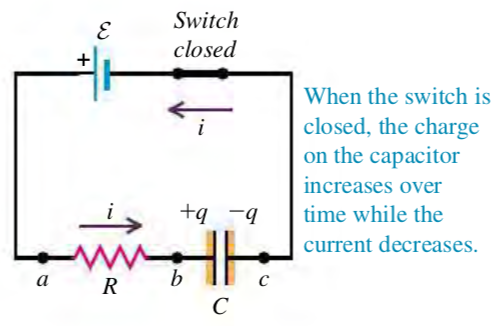
\includegraphics[scale=0.65]{images/RC_circuit.png}}
    \item Suppose the battery has a constant emf of $\mathcal{E}$ and zero internal
        resistance ($r = 0$). Now suppose the capacitor of the circuit is initially
        charged at $t=0$. Then the switch is closed, completing the circuit.
    \item Because the capacitor is initially uncharged, the potential difference $v_{bc}$
        across it is zero at $t = 0$. By Kirchhoff's loop law, the voltage $V_{ab}$
        across the resistor $R$ is equal to the battery $\mathcal{E}$
    \item The initial current through the resistor $I_0$ is given by Ohm's law:
        $I_{0}=\frac{v_{ab}}{R} = \frac{\mathcal{E}}{R}$.
    \item As the capcitor charges, the voltage $v_{bc}$ increases and the potential
        difference $v_{ab}$ across the resistor decreases, corresponding to a decrease in
        current. The sum of these two voltages is constant and equalt to $\mathcal{E}$
    \item Let $q$ represent the charge on the capacitor and $i$ the current of the
        circuit at time $t$ after the switch has been closed. The instantaneous potential
        differences $v_{ab}$ and $v_{bc}$ are:
        \begin{align}
            v_{ab} = iR && v_{bc} = \frac{q}{C}
        \end{align}
    \item After Kirchhoff's loop rule, we havr that:
        \begin{equation}
            \mathcal{E} - iR - \frac{q}{C} = 0
        \end{equation}
    \item The potential drops by an amount $iR$ as we travel from $a$ to $b$ and by
        $\frac{q}{C}$ as we travel from $b$ to $c$. So we find that:
        \begin{equation}
            i = \frac{\mathcal{E}}{R} - \frac{q}{RC}
        \end{equation}
    \item At time $t=0$, when the switch is first closed, the capcitor is uncharged so
        $q=0$. So using this we find that $I_{0} = \mathcal{E} / R$. As the charge $q$
        increases, the term $q / RC$ becomes larger and the capcitor charge approaches
        its final value, which we call $Q_f$
    \item The current decreases and eventually becomes zero. When $i = 0$, we have:
        \begin{align}
            \frac{\mathcal{E}}{R} = \frac{Q_f}{RC} && Q_f = C\mathcal{E}
        \end{align}
    \item We can derive general expressions for charge $q$ and current $i$ as functions of
        time. Since $i$ equals the rate at which positive charge arrives at the positive
        plate of the capacitor, $i = dq / dt$, so
        \begin{equation}
            \frac{dq}{dt} = \frac{\mathcal{E}}{R} - \frac{q}{RC} =
            - \frac{1}{RC}(q - C\mathcal{E})
        \end{equation}
        Which can be rearranged as:
        \begin{equation}
            \frac{dq}{q - C\mathcal{E}} = - \frac{dt}{RC}
        \end{equation}
        integrating both sides we have that:
        \begin{equation}
            \int_0^q \frac{dq^{\prime}}{q^{\prime} - C\mathcal{E}} =
            -\int_0^t \frac{dt^{\prime}}{RC}
        \end{equation}
        Which becomes:
        \begin{equation}
           \ln \bigg(\frac{q-C\mathcal{E}}{-C\mathcal{E}}\bigg) =
           - \frac{t}{RC}
        \end{equation}
        Exponentiating both sides and simplifying:
        \begin{equation}
            \frac{q - C\mathcal{E}}{-C\mathcal{E}} = e^{-t / RC}
        \end{equation}
    \item So for an R-C Circuit, the charging capacitor charge is:
        \begin{equation}
            q = C\mathcal{E}(1 - e^{-t /RC}) = Q_f(1 - e^{-t /RC})
        \end{equation}
    \item The instantaneous current $i$ is just the time derivative of $q$
        \begin{equation}
            i = \frac{dq}{dt} = \frac{\mathcal{E}}{R}e^{-t /RC} =
            I_0 e^{-t /RC}
        \end{equation}
\end{itemize}

\subsection{Time Constant}
\begin{itemize}
    \item After a time equal to $RC$, the current in the R-C circuit has decreased to
        $1 / e$ of its initial value. The capcitor now has reached $(1 - 1 / e) = 0.632)$
        of its final value $Q_f = C\mathcal{E}$. The product $RC$ is therefor a measure
        of how quickly the capacitor charges. This value $RC$ is known as the time
        constant or relaxiont time of the circuit, $\tau$
        \begin{equation}
            \tau = RC
        \end{equation}
    \item When $\tau$ is small, the capcitor charges quickly, while larger values of
        $\tau$ cause for longer charging.
\end{itemize}

\subsection{Discharging a Capacitor}
\begin{itemize}
    \item Suppose after the capacitor has aqcuired a charge $Q_0$, we remove the battery
        from R-C circuit and connect points $a$ and $c$ to an open switch. When the
        switch closes, The capacitor then discharges through the resistor, and its charge
        eventually decreases to zero

        \centerline{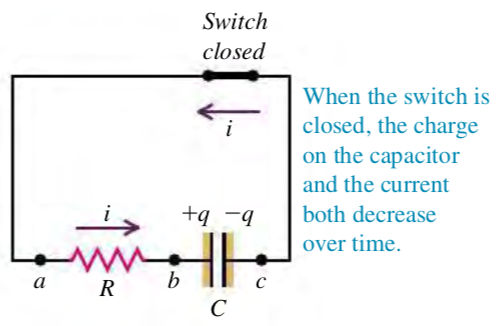
\includegraphics[scale=0.65]{images/discharging_circuit.png}}
    \item Kirchhoff’s loop rule when $\mathcal{E} = 0$ is:
        \begin{equation}
            i = \frac{dq}{dt} = - \frac{q}{RC}
        \end{equation}
    \item The current $i$ is now negative, this is because positive charge $q$ is leaving
        the left capacitor plate, so the current is in the direction opposite to that in
        the diagram.
    \item To find q as a function of time, integrate:
        \begin{equation}
            \int_{Q_0}^{q} \frac{dq^{\prime}}{q^{\prime}} =
            - \frac{1}{RC} \int_{0}^{t} dt^{\prime}
        \end{equation}
        Which becomes:
        \begin{equation}
            \ln \frac{q}{Q_0} = - \frac{t}{RC}
        \end{equation}
    \item So the capacitor charge in a discharging circuit can be modeled with the
        following function:
        \begin{equation}
            q = Q_0 e^{-t / RC}
        \end{equation}
    \item The instantaneous current i is the derivative of this with respect to time
        \begin{equation}
            i = \frac{dq}{dt} = - \frac{Q_0}{RC} e^{-t / RC} = I_0 e^{-t /RC}
        \end{equation}
    \item While the capacitor is charging, the instantaneous rate at which the battery
        delivers energy to the circuit is $P = \mathcal{E}i$
    \item The total energy supplied by the battery during charging of the capcitor equals
        the battery emf $\mathcal{E}$ multiplied by the total charge $Q_f$
\end{itemize}

\end{document}
